\documentclass[conference]{IEEEtran}
%\IEEEoverridecommandlockouts
% The preceding line is only needed to identify funding in the first footnote. If that is unneeded, please comment it out.
\usepackage{cite}
\usepackage{amsmath,amssymb,amsfonts}
%\usepackage{algorithmic}
\usepackage{graphicx}
\usepackage[inline]{enumitem}
\usepackage{textcomp}
\usepackage{xcolor}
\usepackage{csquotes}
\usepackage{fancyvrb}
\usepackage{verbatim}
\usepackage{algpseudocode}
\usepackage{url}
\usepackage{listings}
\usepackage{tabularx}
\usepackage{comment}
\usepackage{flushend}

% don't use all cap for algorithmic 
\algrenewcommand\textproc{}

\newcommand\hl[1]{\colorbox{red!10}{#1}}
\newcommand{\ajay}[1]{{\color{magenta} {\bf Ajay:} #1}}
\definecolor{xxxcolor}{rgb}{0.8,0,0}
\definecolor{maroon}{RGB}{128,0,64}
\definecolor{darkgreen}{RGB}{0,128,64}
\newcommand{\ignore}[1]{}
\newcommand{\chcomment}[1]{{\color{xxxcolor} {\bf Charith: [}\emph{#1}{]}}}

%%%%%%%%%% use lower capse for table caption
\usepackage{etoolbox}
\makeatletter
\patchcmd{\@makecaption}
  {\scshape}
  {}
  {}
  {}
\makeatother
%%%%%%%%%%%

\def\BibTeX{{\rm B\kern-.05em{\sc i\kern-.025em b}\kern-.08em
    T\kern-.1667em\lower.7ex\hbox{E}\kern-.125emX}}
    
    
\begin{document}

\title{A Benchmark Suite and Measurement Framework for Validating x86-64 Basic Block Cost Models}

%\author{\IEEEauthorblockN{1\textsuperscript{st} Given Name Surname}
%\IEEEauthorblockA{\textit{dept. name of organization (of Aff.)} \\
%\textit{name of organization (of Aff.)}\\
%City, Country \\
%email address}
%}

\maketitle

\thispagestyle{plain}
\pagestyle{plain}

\begin{abstract}
%Modern microprocessors have undergone decades of hardware optimizations.
%For example, modern x86-64 microprocessors employ sophisticated
%instruction execution paths with heavily pipelined,
%out-of-order, super-scalar execution units that are highly complex.
%Producing code that
%exploits and optimizes for this underlying execution environment requires careful
%modelling of the microprocessor functionality. To achieve this, modern compilers employ processor models that predict
%the cost of
%executing a set of instructions to perform backend optimizations such as instruction
%selection, register allocation, instruction scheduling etc.
%\ajay{The lines till here sound a bit repetitive. We are not saying anything concrete here. All we are saying is microprocessors are complex}.
%\ajay{Also, mentioning x86\_64 as an example is a bit misleading. Because we do only for x86\_64. We should start directly with - Modern x86\_64 employs}.
%However, these cost models receive less attention than optimizations themselves.
Modern x86 processors have complex performance characteristics due
to micro-architectural optimizations such as \chcomment{pipelining, super-scalar,} out-of-order executions and micro-op fusions.
To reduce the complexity of optimizing for these processors,
many optimization techniques, manual or automatic, use cost models
to abstract away target machines.
Inaccurate models can cause misoptimizations.
There are known, sometimes significant issues of
cost models in production compilers such as LLVM\cite{llvm} and machine code analyzers
written by processor vendors themselves such as IACA\cite{iaca}.
IACA has been shown in some cases to deviate from the measured throughput
of a basic block of instructions by more than 2x.
Despite this, there is no standard, systematic approach or tooling
to perform validation and tuning of processor cost models.

In this paper, we present the necessary tooling and a benchmark suite
for validating and tuning cost models of x86-64 basic blocks.
Our benchmark suite contains more than 300,000 \chcomment{should have the number for the entire suite}
basic blocks extracted from a wide range of applications.
We describe our techniques to profile arbitrary basic blocks automatically and accurately;
which entails much more than simply measuring the latency of an unrolled basic blocks;
in fact our ablation study shows that the profiling \textit{without} some of our measures
ranges from crashing to obtaining results that are orders of magnitude away from the ground truth.\chcomment{
Something on how hard measurement is?}
We analyze the benchmark suite and show how and where popular
cost models used by static predictors such as llvm-mca, IACA, Ithemal and
OSACA\cite{osaca} deviate from the ground truth measured data.
We show that in certain classes of basic blocks
(e.g. vectorized numerical kernels) even the most accurate
model is on average more than 30\% away from the ground truth.
Furthermore, our dataset can be used as training data for learning-based cost models, such as in Ithemal.

%In addition to cost model validation,
%our dataset and the profiling infrastructure is useful
%for data-driven cost model construction\cite{ithemal}.

%In spite of this, compiler cost models undergo low levels
%of validation and scrutiny due to the lack of tolling and
%test suites that generate validation data.


% Modern super-scalar out-or-order processors are complex objects.
% To reduce the complexity of optimizing for these processors,
% many optimization techniques, manual or automatic, use cost models
% to abstract away target machines.
% Cost models however receive less attentions than optimizations,
% and inaccurate models can cause miss optimizations.
% There are known, sometimes significant issues of
% cost models in production compilers such as LLVM\cite{llvm,goslp}.
% Even IACA, Intel's own throughput predictor has
% been shown in some cases to deviate from measured throughput
% by more than 100\%.

% Despite the importance of existing cost models,
% to this day there is no standard, systematic approach 
% to perform cost model validation and tuning.
% We describe a benchmark for validating performance 
% models of x86 basic blocks.
% Our dataset contains more than three hundred thousand
% basic blocks extracted from a wide range of applications.
% We describe our technique to profile the throughput
% of these basic blocks automatically and accurately.
% We automatically classified our basic blocks by their use
% of CPU resources and evaluated accuracy of existing cost models
% for different classes of basic blocks. 
% We showed that in certain classes of basic blocks 
% (e.g. vectorized numerical kernels) even the most accurate
% model is on average more than 30\% away from the ground truth.
% In addition to cost model validation,
% our dataset and the profiling infrastructure is useful
% for data-driven cost model construction\cite{ithemal}.
\end{abstract}
\begin{IEEEkeywords}
performance models, basic block profiler, x86-64, basic block benchmark suite
\end{IEEEkeywords}
\section{Introduction}
Many optimizations, whether manual or automatic,
benefit from performance models.
Static performance models such as IACA lessen programmers
the burden of isolating performance kernels from
the rest of the applications,
and of properly implementing micro-benchmark. Many compiler optimizations
use cost models of one form or another:
a typical automatic vectorizer, for instance,
use one to estimate the cost of vector packing
in the presence of irregular memory accesses~\cite{goslp};
instruction schedulers uses one to model the latency
and throughput of instructions~\cite{llvm-sched,gcc-sched}.

Cost models however often take a back seat to “actual” optimizations,
despite the accuracy of former ensures the effectiveness of latter.
For instance, Mendis et al.\cite{goslp}
recently published a technique to perform optimal\footnote{
Witch certain caveat.
In particular their formulation is optimal
only when the target machine only has vector-width of 2}
SLP Vectorization\cite{slp} that
incurred slowdown in some instances due to the inaccuracy of 
LLVM's cost models.
Without a comprehensive benchmark to pinpoint the weakness of their models,
developers cannot systematically improve these cost models;
model parameters
such as the throughput of individual instructions
are sometimes chosen haphazardly;
consider following quote taken from a commit message from LLVM\cite{llvm}
regarding its cost model\footnote{
https://reviews.llvm.org/D46276.
}:
\begin{quote}
X86's fix to avoid SDIV/UDIV vectorization is clumsy
(multiplying the vector costs x20)
and appears to have been implemented before the cost of
scalarization was being realistically accounted for...
\end{quote}

We describe a benchmark for validating performance models
of x86 basic blocks.
In this work we focus on throughput prediction.
We make the following contributions:
\begin{enumerate}
\item We collected basic blocks from a wide range of domains.
This data set, together with additional profile information we collected,
can be used to design and validate low level optimizations
such as backend peephole optimizers,
in addition to its primary purpose of model validation.

\item We describe a fully automatic technique
for measuring the throughput of basic blocks extracted 
from raw binaries.
This is much more than simply measuring the latency of an unrolled basic block
since code snippets with memory accesses (and most do)
generally cannot be executed safely
outside of the context of their source applications.
We have used this technique to profile the throughput of more than 2 million basic blocks.
Our methodology, when implemented, is accurate and fast.
Depends on the context -- 
if a developer is only interested in the performance of a code snippet
but not how constituent instructions contribute to the final
throughput -- our tool outperforms IACA in both speed and accuracy.

\item We automatically classified the basic blocks
by their usage of different execution ports.
This classification allows developers to pinpoint weakness
of their performance models.
Maintainers of an automatic vectorizer, for instance,
can use this to fine-tune cost models
of vectorized basic blocks.

\item We evaluated four existing cost models:
IACA, llvm-mca -- 
which exposes LLVM’s internal optimization cost models,
OSACA\cite{osaca}, and Ithemal\cite{ithemal}.
We breakdown the strength and weakness of these cost models on
different classes of basic blocks;
e.g. we show that all such tools
have average error higher than 30\% 
when used to analyze numerical kernels running on Haswell machines.



\end{enumerate}
\section{Background}

\subsection{Existing Performance Models}
\label{sec:perf-models}

IACA~\cite{iaca} (Intel Architecture Code Analyzer) is a static analyzer
developed by Intel. It has support for Intel micro-architectures
since Nehalem.
Given a machine code snippet, IACA estimates the average number
of cycles it costs to execute the given code in an infinite 
loop.
Unlike its alternatives, IACA takes advantage of its knowledge
of Intel's proprietary processor optimization---such as zero-idioms and micro-op fusions---to make better 
predictions.

llvm-mca~\cite{llvm-mca} is a similar tool inspired by IACA. 
Implemented as an out-of-order super-scalar simulator,
it uses parameters (e.g., instruction throughput)
supplied by LLVM\cite{llvm}'s backend scheduling model.
Reusing of the scheduling model is an explicit design choice
made to expose LLVM's cost model for testing.
Thus the accuracy of llvm-mca has a bearing on
that of LLVM's scheduling model.

OSACA\cite{osaca} is an analyzer developed as the open-source
alternative to IACA. It is similar to llvm-mca in that
it is implemented as a parametrized out-of-order simulator---in
this case, the parameters come from the measured throughput
and latency data for individual instructions.

Ithemal\cite{ithemal} is a basic block throughput predictor
implemented as a deep neural network. Unlike other models discussed so far, 
tools, Ithemal is not a simulator in the sense that it outputs
a single throughput prediction for each input basic block
without reporting an interpretable execution trace.

Production compilers such as LLVM\cite{llvm} and GCC typically use cost models 
to guide optimizations.
Unlike ``user-facing'' models such as IACA or llvm-mca, these cost models typically
model the costs at the instruction level, rather than at whole basic block level.
These compilers also use multiple cost models.
LLVM, for instance uses (at least) three cost models: 
a generic, per-instruction IR cost model in its middle-end IR~\cite{llvm-cost};
one that captures the information required for instruction scheduling,
(i.e. the scheduling model~\cite{llvm-sched}, also used by llvm-mca);
and another one that models the cost of register uses---such as cost of loads
and register-to-register transfer---in register allocation~\cite{llvm-reg}.
GCC similarly employs analogous models~\cite{gcc-cost,gcc-sched}.
Out of the models discussed so far, to our best knowledge, 
the scheduling model of LLVM is the only one exposed by an interface
(in this case, llvm-mca) for testing in isolation from its client optimizations.
% TODO: can we make a stronger statement saying given our work, we think
% other models should be exposed as well?


\vspace{1em}
\noindent{\bf Modeling Assumptions.}
All of cost models discussed above make the following assumptions about the execution context
of the code they are modeling
\begin{itemize}
    \item All memory accesses hit the L1-cache.
    \item All instructions reside in the instruction cache.
    \item The execution is unaffected by context switches and interrupts.
\end{itemize}

\subsection{Existing Validation Tools and Profilers}
We briefly discuss existing tools and sources used by developers to validate
processor performance  models.
There are roughly two categories of these sources:
\begin{enumerate*}
\item per-instruction cost table tabulated either by
consulting the manual or manual benchmarking;
\item machine code profiler for running microbenchmarks.
\end{enumerate*}

\textbf{Per-instruction Latency/Throughput Tables}
These datasets are created either by scraping hardware manual or
by manual profiling 
(to obtain the real instruction latency or throughput).
Current sources of per-instruction information are incomplete and sometimes inaccurate~\cite{uops}. 
More importantly, they do not lead directly to validating performance model at basic block level or more.
Although in general, it is possible to estimate the throughput of 
a basic block by inferring the scheduling of its instructions based on their
port usage---this is the approach taken by llvm-mca~\cite{llvm-mca} and OSACA\cite{osaca}---this
it is incomplete and does not take microarchitectural
optimizations that could alter the ``normal'' execution paths into account. 
Examples of these optimizations include micro-op fusion and zero-idioms.
Therefore, IACA\cite{iaca} is generally recognized as the more accurate analyzer
compared to its alternatives since it can exploit
private optimizations employed by Intel's processors.

Intel's manual\cite{intel-manual} provides the throughput and latency
of frequently used instructions.
Agner Fog\cite{agner} similarly provides a table of instruction throughput and latency.
Google's EXEgesis team~\cite{exegesis} provides a tool that can automatically extract
machine-readable instruction specifications from Intel's manual.
llvm-exegesis, designed by the same team, is a tool that determines
the latency of an input instruction opcode\footnote{
Currently the tool is limited to instructions that does not touch memory or floating point registers} 
by automatically generating a micro-benchmark that measures the opcode's average latency;
some LLVM's developers use the tool to validate LLVM's scheduling model.

Abel and Reineke\cite{uops} recently published their methodology
to reverse engineer the detailed mapping from each instruction to the
combination of execution ports
that these micro-ops can use.
They build instruction-to-port mapping using automatically generated micro-benchmarks.
Based on this mapping, they infer the steady-state scheduling of constituent
micro-ops for an instruction and calculate the instruction throughput based on
this inferred schedule.

\textbf{Machine Code Profiler} These tools allow users to perform
detailed microbenchmarking and are used by compiler writers manually
to verify compiler cost models.
These profilers are, however, unsuitable for our work---i.e., profiling
a large set of arbitrary basic blocks for systematic validation.
They require user intervention to profile arbitrary basic blocks. Most notably,
user annotation is needed to allocate memory and
initialize memory-addressing registers to prevent crashing.

Agner Fog~\cite{agner} provides a script to profile small code snippets.
The script reports the number of cycles as well as performance statistics such as 
the number of cache misses.
The script assumes that it is the user's responsibility to ensure
the successful execution of the benchmark;
for instance, the user is expected to allocate memory and initialize pointers.

nanoBench~\cite{nanobench} is a profiler similar to that of Agner Fog's~\cite{agner},
with two notable improvements.
It allows the user to specify which processor-specific hardware
to measure---in addition to cycle-counter. It also supports profiling in kernel-mode,
removing potential noise due to context-switches and interrupts.

% TODO:
% 1. talk about compiler cost models (both LLVM and GCC), mention that there is a chicken and egg issues
% 2. talk about stuff like agner fog's script
\section{Basic Block Profiling}
The standard methodology for measuring the throughput of a basic block
is to measure the latency of $n$ unrolled copies of the basic block
and divide that latency by $n$.
One of the commonly used latency measurement tool is Agner Fog's measurement script~\cite{agner}.
This script is straightforward. 
It uses the core cycle counter to measure the latency of an unrolled basic block and
does not modify the basic block's execution context in any way.
The first row of Table~\ref{tab:full-ablation} presents the results of applying
this methodology to our benchmark suite. 
The result is that this methodology is only able to {\em successfully profile}\footnote{
We say a basic block is successfully profiled when it meets all of the following criteria:
The basic blocks can be successfully executed by our profiler;
the execution does not incur any cache misses (including data and instruction cache);
we are able to reproduce the measurement.
} 16.65\% of our basic blocks.


Our goal is to maximize the number of basic blocks that execute without crashing, subject to the constraint that their executions satisfy our performance modelling assumptions (Section~\ref{sec:perf-models}) .

We first describe a technique to map all virtual memory pages accessed by a basic block
to a single physical page before the execution of this basic block;
this achieves two objectives: the basic blocks can then be executed without crashing,
and all of the memory accesses hit the L1 data cache.
This allows us to execute most basic blocks (see Table~\ref{tab:full-ablation})
but does not guarantee that there is no instruction cache
miss (an assumption of all existing performance models),
which can become an issue when one attempts to profile large basic blocks using
the standard unrolling-based throughput profiling.
In particular, the issue with the standard approach is that the unroll factor
has to be large enough to hide the latency of the first and last few iterations,
but such an unroll factor can cause instruction cache misses for large basic blocks,
violating our modeling assumptions.
We describe our technique to profile basic blocks with smaller
unroll factors while providing accurate steady state throughput estimation.
Table~\ref{tab:full-ablation} shows the percentage of basic blocks
we are able to profile using these two techniques.

We additionally discuss two rare events --
gradual underflow of floating points and unaligned memory accesses -- 
that can significantly affect profile fidelity;
we avoid the former entirely and detect the occurrence of the latter.

\subsection{Handling memory accesses}\label{sec:mapping}
We now describe our technique to execute arbitrary, memory-accessing basic blocks
without user intervention.
We first show a motivating example.
Consider the basic block in figure \ref{fig:mem-ex},
which is used to compute the CRC code of input bytes in Gzip.
Highlighted instructions shows the flow of pointer values;
essentially \textit{bits} of \verb|%rdx| are used to index into a lookup table, 
and the content of which is then used in the next iteration to 
update \verb|%rdx|.
How would one profile the throughput of this basic block?
Without the original application context,
this basic block \textit{cannot} be directly executed.
Developers of Gzip familiar with this piece of code could 
properly setup a micro-benchmark by reproducing the
relevant lookup table used by this code snippet,
but such an approach would not scale to the hundreds of 
thousands of basic blocks in our data set, most of which contain memory accesses.
We needed some way to automatically generate the benchmarking environment
without \textit{a priori} knowledge/assumption of the code being profiled.
\if 0

    add rdi, 1
    #hl{mov eax, edx}
    shr rdx, 8
    #hl{xor al, [rdi - 1]}
    movzx eax, al
    #hl{xor rdx, [8*rax + 0x4110a]}
    cmp rdi, rcx
\fi
\begin{figure}[h]
\begin{Verbatim}[commandchars=\#\{\}]
    
    add $1, %rdi
    #hl{mov %edx, %eax}
    shr $8, %rdx
    #hl{xor -1(%rdi), %al}
    movzx %al, %eax
    #hl{xor 0x4110a(, %rax, 8), %rdx}
    cmp %rcx, %rdi
\end{Verbatim}
\caption{Inner loop body of updcrc from Gzip.
This basic block cannot be directly executed because
of its memory accesses.}
\label{fig:mem-ex}
\end{figure}

\begin{figure}
\begin{algorithmic}

\Function{measure}{}
    \State $page \gets \Call{getRegisterValue}{rax}$
    \State $\Call{mmapToChosenPhysPage}{page, ...}$
    \State $\Call{initialize}{}$
    \State $\Call{executeUnrolledBasicBlock}{}$
    
    \Comment{After this point all memory accesses made by the basic block is legal
    and goes to L1 cache}
    
    \State $begin \gets \Call{readPerformanceCounters}{}$
    \State $\Call{initialize}{}$
    \State $\Call{executeUnrolledBasicBlock}{}$
    \State $end \gets \Call{readPerformanceCounters}{}$
    \State $\Call{analyzeAndReportCounters}{begin, end}$
\EndFunction

\Function{monitor}{}
    \State $pid \gets \Call{launchAndMonitor}{measure}$
    \State $numFaults \gets 0$
    \While{$true$}
        \State $memAddr \gets \Call{interceptSegFault}{pid}$
        \If{$\Call{isValidAddr}{memAddr}$}
            \State $page \gets \Call{getPageAddr}{memAddr}$
            \State $\Call{setRAX}{pid, page}$
            \State $\Call{setInstructionPointer}{pid, measure}$
            \State $\Call{resumeProcessExecution}{pid, measure}$
            \State $numFaults \gets numFaults + 1$
        \EndIf
        \If{$numFaults > maxNumFaults$}
            \State $\Call{kill}{pid}$
            \State \textbf{break}
        \EndIf
    \EndWhile
\EndFunction

\end{algorithmic}

\caption{Pseudocode of the our profiling routines. 
\textit{measure} runs in a child process monitored by
\textit{monitor}.
We execute an input basic block twice.
The first execution is used to discover virtual pages accessed
by the basic block, which are the then mapped to a single physical page.
We collect performance statistics in the second execution.}
\label{fig:code}
\end{figure}

We now describe our solution to profile arbitrary basic blocks with memory accesses.
Our profiling algorithm consists of two steps.
\begin{enumerate*}
\item We first the identify the virtual pages accessed by
the basic block 
and map those virtual pages to a single physical page.
\item After the appropriate mappings are created,
the unrolled basic block is then executed normally under
the new page mapping.
\end{enumerate*}

\textbf{Mapping pages to avoid SegFaults}
In addition to making all the memory accesses made by the basic block valid,
the mapping stage also ensures that all memory accesses go to the same physical page and hence stay in the L1 data cache. 
Figure~\ref{fig:code} shows the algorithm we use to do the page mapping.
Mapping is done by executing the unrolled basic block in a forked process
 monitored by a parent process using \verb|ptrace|.
Each attempt to access an unmapped virtual page is intercepted by
the monitoring process, which then instructs the 
executing process to create the appropriate mapping
and to restart execution from the \textit{beginning}
with all registers, memory values,
as well as the flag registers reinitialized.
Re-initialization is done to ensure that in the final measurement
stage the trace of memory addresses computed by the 
unrolled basic block is \textit{identical} to that from the mapping stage.
An alternative we considered was using a single process for both execution
and monitoring, but we ultimately discarded this alternative due to
its complexity.\footnote{Unmapping all the libc pages forces us to write all the code in assembly.}


%We use this methodology as the baseline and compare it with three techniques.
%\begin{enumerate}
%    \item Naive memory mapping.
%    
%    This is an naive attempt to reduce the number of crashes due to segmentation faults.
%    We try to allocate as much memory as possible in the hope that 
%    a basic block only try to access the allocated memory.
%    Since we want to avoid cache misses, we only allocate 32KB of memory (size of the L1 cache).
%    We also initialize all general purpose registers to point to the allocated memory.
%    
%    \item Mapping all virtual pages accessed by a basic block to a single physical page 
%    (while using identical initialization).
%    
%    This is our full solution to executing basic blocks with ``random'' memory traffic.
%    We describe how we construct this mapping in more detail in Section~\ref{sec:mapping}.
%    We are able to profile most basic blocks using this technique alone (90\%).
%    
%    \item More intelligent unrolling of basic blocks.
%    
%    This is our technique for profiling large basic blocks that could cache instruction cache misses
%    if profiled naively.
%    A common practice of basic block profiling is unrolling the basic block
%    multiple times and measuring the latency of executing the unrolled code;
%    We show that naively applying this technique to large basic blocks
%    leads to mis-profiling by overflowing instruction cache,
%    and we show how we are able to use smaller unroll factors that gives
%    accurate throughput estimation.
%\end{enumerate}

%Table~\ref{tab:ablation} shows the effect of incrementally applying
%our techniques to measure a basic block sampled from 
%TensorFlow~\cite{tensorflow}'s CNN training benchmark.
%As demonstrated, without some of these techniques,
%the results vary from obtaining no throughput due to crashes or
%estimations that are two orders of magnitude away from the 
%actual throughput.
%
%

\begin{table}
\begin{tabular}{
|p{0.4\columnwidth}|p{0.45\columnwidth}|}
\hline
\textbf{(Additional) Technique} & \textbf{Percent of Basic Blocks Profiled} \\
\hline
None & 16.65\% \\

\hline
Mapping all accessed pages & 91.28\% \\

\hline
More intelligent unrolling & 94.24\% \\

\hline
\end{tabular}
\\
\caption{Ablation study showing the effect of incrementally applying our measurement techniques.}
\label{tab:full-ablation}
\end{table}


\subsection{Deriving throughput from measurement}
We use IACA's definition of throughput, i.e. 
the average number of cycles required to execute a basic block 
at steady state.
\footnote{Note that this definition is the inverse of the textbook definition of throughput.}

The basic strategy one usually takes to measure basic block throughput
is unrolling a basic block multiple times and dividing the latency of the
unrolled basic block by the unroll factor.
The formula for estimating the throughput using this approach is shown
in equation~\ref{eq:naive}, where $u$ is a large unroll factor
and $\mathit{cycles}(b,u)$ is the number of cycles taken to execute basic block $b$
unrolled $u$ times.
\begin{equation}
\mathit{throughput}(b) \approx \frac{\mathit{cycles}(b,u)}{u}
\label{eq:naive}
\end{equation}
Compared to running the basic block inside a loop,
unrolling has an advantage in that the measurement is not polluted by
overhead incurred by looping.
A typical unroll factor is 100\cite{ithemal,uops}.
Such a high unroll factor can however incur significant
L1-instruction cache misses for large basic blocks
(e.g. the already unrolled inner-loop body of a GEMM kernel).

The issue with unrolling naively is that,
an unroll-factor small enough to 
avoid instruction cache misses is 
insufficient to hide the latency of the first few iterations.
We thus adopted a different strategy to cope with large basic blocks.
Equation~\ref{eq:new} shows the formula we use to estimate throughput.
We unroll each basic block with two different unroll factors.
These factors should be large enough 
to warm-up the processor into a steady state.
We then measure the latency of the two unrolled basic blocks,
calculate the difference in the measurements, and divide it 
by difference of the unroll factors.
The resulting number is the throughput of the basic block.
\begin{equation}
\mathit{throughput}(b) \approx 
\frac{\mathit{cycles}(b, u) - \mathit{cycles}(b, u')}{u-u'}
\label{eq:new}
\end{equation}

\begin{equation}
\mathit{cycles}(b, u') \approx 
\mathit{cycles}(b, u) + \frac{\mathit{throughput(b)}}{u'-u}
\label{eq:new-rearranged}
\end{equation}
Equation~\ref{eq:new} is an re-arrangement of equation~\ref{eq:new-rearranged},
which is derived from the following observation:
if unroll factors $u$ and $u'$ are large enough
to get the processor into a steady state,
then the additional $u'-u$ (suppose $u' > u$) iterations will be processed at 
the rate of steady state throughput.

The only requirement for unroll factors $u$ and $u'$ in equation~\ref{eq:new}
is that they are large enough to get the processor into a steady state,
while the unroll factor $u$ in equation~\ref{eq:new} has to be additionally
large enough to amortize the cost of the first few iterations.
Being able to profile with smaller unroll factors is essential
for large basic blocks that typically show up in numerical kernels where
some hot inner loops are unrolled.


\subsection{Enforcing Modeling Variants}\label{sec:invariants}
We guarantee that each measurement satisfies the following modeling assumptions:
\begin{enumerate*}
    \item Every memory accesses leads to an L1 data cache hit. 
    \item Measurements are free of interrupts, context switches,
    and hyper-threading.
\end{enumerate*}
These are the same assumptions made by existing models;
Admittedly many of the memory accesses in deployed programs do not hit the L1 data cache.
We nonetheless make sure that during our measurement all memory accesses hit the L1 data cache for compatibility with existing models.
%We acknowledge that the throughput of the basic blocks depends on the program context, but 
%the throughput of these basic blocks (i.e. those with memory accesses)
%is inherently dependent on the program execution context.

To enforce these assumptions, we monitor the following statistics in addition to core cycle counts, and reject a measurement if one of these statistics is not zero. 
\begin{enumerate}
    \item L1 Data Cache Read Misses
    \item L1 Data Cache Write Misses
    \item L1 Instruction Cache Misses
    \item Context Switches
\end{enumerate}
We measure the cache misses with hardware performance counters, 
and we use one of the system calls provided by Linux to track the number of context switches. 
Each \textit{unrolled} basic block is timed 16 times by default,
and we accept a basic block for further analysis only if the basic block has at least 
8 \textit{clean}, identical timings.
All basic blocks are measured in machines with hyper-threading disabled.
We count the elapsed cycles by reading the core cycle counter.
Unlike the reference cycle counter or the time-stamp counter, the core cycle counter is invariant
to performance scaling.
As discussed in~\ref{sec:mapping}, we map all virtual pages accessed by 
a basic block to a single physical page.
The L1 data caches of recent Intel microarchitectures are virtually indexed and physically tagged. 
As a result all these virtual pages are identical for the cache and it sees as if the same page is accessed over and over again leading to perfect cache hits 
(our solution would not work for architectures using virtually tagged caches).

\subsection{Additional measurement optimizations}
We make additional optimizations to further increase our chance
of successfully obtaining clean measurements.

\textbf{Initialization} 
Prior to the mapping-run,
we unmap all pages (except those containing the basic block).
This allows us to ensure that all the memory accesses go to our single 
physical page and not to some previously mapped address (like libc).
The physical page is
always initialized to be filled with a “moderately sized” constant
(we used \verb|0x12345600| in our experiments)
to accommodate for indirect memory accesses.
To see why this is necessary,
consider a basic block that first loads a pointer $p$ from memory
and then de-references $p$.
If the value of $p$ is too low (e.g. 0)
or too high
(i.e. bigger than the maximum memory that
a user space program is allowed to addressed),
we will not be able to map the virtual page pointed by $p$.
All general-purpose registers are initialized similarly.

\textbf{Handling Subnormal Numbers}
General speaking -- aside from division
and specialized instructions such as \verb|sqrt|
-- floating point instructions have constant timings
except when the inputs of the operations are subnormal numbers.
In our experiments where we encountered subnormal numbers,
floating point operations can be slowed down by up to 20x.
To ``normalize'' our timing, we configured \verb|MXCSR| register
to disable gradual underflow.
We found that 334 ($0.1\%$) basic blocks would have been affected by 
gradual underflow if we had not taken this measure.


\textbf{Detecting unaligned accesses}
If the address being 
accessed crosses a cache line boundary, 2 cache lines have to be read/written. This can cause
an order of magnitude slowdown in the measurements. We do not want these measurements to 
pollute our dataset. So, we introduce another filter into our measurement tool. We use the 
\verb|MISALIGNED_MEM_REFERENCE| counter to measure the number of stores and loads that cross a cache line boundary for 
each basic block. If a basic block has even a single such load or store, we drop that basic block. 
This filter ended up dropping 553 ($0.183\%$) basic blocks. 

\begin{table}
\begin{tabular}{
|p{0.2\columnwidth}|p{0.18\columnwidth}|p{0.18\columnwidth}|p{0.18\columnwidth}|}
\hline \textbf{(Additional) Optimizations} &
\textbf{Measured Throughput} &
\textbf{L1 D-Cache Misses} &
\textbf{L1 I-Cache Misses} \\

\hline
None & Crashed & N/A & N/A \\

\hline
Page mapping & 6377.0 & 956 & 0 \\

\hline
Single physical page & 2273.7 & 0 & 0 \\

\hline
Disabling gradual underflow & 65.0 & 0 & 35 \\

\hline
Using smaller unroll factor & 59.0 & 0 & 0\\

\hline
\end{tabular}
\\
\caption{Measured throughput for a sample basic block when
different measurement optimizations are incrementally applied.
The basic block is extracted from one of the critical 
inner loop body of TensorFlow\cite{tensorflow}'s CNN training benchmark.}
\label{tab:ablation}
\end{table}
\section{Basic Block Collection and Classification}
Modern microarchitectures employ various optimizations:
pipelining, super-scalar execution, dependency breaking zero-idioms, micro-op fusion, etc.
Some of these optimizations are not documented and are proprietary.
To validate performance models effectively, one would need to take
all of these optimizations into account.

A wide range of code sequences are needed to reveal a predictor's 
weakness (or the lack of) in modelling the complex interaction of 
individual instructions in modern hardware. 

\subsection{Basic Block Collection}
In this work, we selected the source applications of our basic blocks with two goals:
\begin{enumerate*}
    \item The set of applications should cover a diverse range
of domains to represent real world workloads
    \item Their basic blocks should reflect usage that concerns typical users of a performance model;
    compiler developers deal with
    basic blocks from general purpose programs,
    which have different characteristics
    than those from 
    high performance kernels. 
\end{enumerate*}
Table~\ref{tab:apps} shows the applications from which we extracted basic blocks.

\begin{table}
\begin{tabular}{|p{0.2\columnwidth}|p{0.3\columnwidth}|p{0.3\columnwidth}|}
\hline
\textbf{Application} & \textbf{Domain} & \textbf{\# Basic Blocks} \\

\hline
OpenBlas & Scientific Computing & 19032 \\

\hline
Redis & Database & 9343  \\

\hline
SQLite & Database & 8871 \\

\hline
GZip & Compression & 2272 \\

\hline
TensorFlow & Machine Learning & 71988 \\

\hline 
Clang/LLVM & Compiler & 212758 \\

\hline
Eigen & Scientific Computing & 4545 \\

\hline
Embree & Ray Tracing & 12602 \\

\hline
FFmpeg & Multimedia & 17150 \\

\hline
\multicolumn{2}{|l|}{Total}  & 358561 \\


\hline
\end{tabular}
\\
\caption{Source applications of basic blocks}
\label{tab:apps}
\end{table}

We selected Clang/LLVM\cite{llvm} (compiler),
Redis (in-memory database), SQLite (database), and Gzip (compression)
to collect basic blocks that represent
applications that are written in general purpose languages
like C and C++.
Basic blocks from these programs
typically have high memory traffic, and are usually not-vectorized.
We chose these applications because they are some of the most used
applications today; they are well tuned for performance;
and they all have sophisticated use of algorithms and data structures,
giving us a large source of diverse basic blocks.

Next, we selected following applications that use hand-optimized high performance kernels:
OpenSSL~\cite{openssl} (cryptography), OpenBLAS~\cite{openblas}, Eigen~\cite{eigen} (scientific computing),
TensorFlow\cite{tensorflow} (machine learning),
Embree\cite{embree} (rendering), and FFmpeg (multimedia).
OpenSSL, OpenBLAS, and FFmpeg use handwritten assembly for performance critical inner loops.
Embree is written in ispc\cite{ispc}, a data parallel language
designed specifically to target Intel's vector extensions.

We collected basic blocks from these applications using
a dynamic analysis implemented in DynamoRIO\cite{dynamorio},
which allows us to record every basic block
executed at runtime.
We opted for dynamic analysis rather than static disassembly
because precise static disassembly of x86 binaries
is undecidable~\cite{disassembly-undecidable}.
We discovered in our experiments cases where
static disassemblers cannot distinguish padding bytes from instructions.
We use the official benchmarking input of these applications\footnote{
Except for FFmpeg and Gzip, which to the best of our knowledge do not have
official benchmarks. For these two applications we use inputs
from https://openbenchmarking.org.
} to simulate realistic execution when recording the basic blocks.
We evaluated Eigen on two sparse linear algebra workloads:
sparse matrix-matrix multiplication (SPMM) and 
sparse matrix-vector multiplication (SPMV).

\subsection{Basic Block Classification}\label{classification}
We additionally classify the basic blocks by their use of processor resources.
This classification, as shown in section~\ref{results},
allows one to compare the prediction accuracy of different types of basic blocks 
(e.g. numerical kernel vs bit-manipulation).

We classify the basic blocks as follows.
The high-level approach we took was to first,
\begin{enumerate*}
\item map each basic block to a vector representation
that reflects its usage of hardware resources,
\item and then cluster the basic blocks by their vector representations.
\end{enumerate*}

Using results from Abel and Reineke~\cite{uops},
we compute a port-combination mapping for each instruction.
For instance,
the port-combination mapping for \verb|xor rax, rbx| in Haswell
is $\{ p0156 \rightarrow 1 \}$ (using Abel and Reineke's notation);
in other words, this instruction is implemented 
with a micro-op that can be executed at port-0, 1, 5, and 6.
In Haswell, there are 13 such port combinations for all user-level instructions.

After translating each instruction to its micro-ops and port combinations, we used Latent Dirichlet Allocation (LDA)~\cite{lda} to build a \emph{topic model}
that assigns a category to each micro-op based on the micro-op's port combination and which basic block it is contained in.
We performed \emph{Bayesian inference} to infer the category for each micro-op
using SciKit Learn's default implementation of stochastic variational inference for LDA\cite{lda},
with 6 categories and the parameter values $\alpha = 1/6$ and $\beta = 1/13$. 
We then computed the most common category for each basic block, taking this to be the category of the basic block itself.
Table~\ref{tab:categories} labels each category with which class of instructions it corresponds to.
Note that LDA does not natively label the categories;
we have manually labelled the categories by manual inspection.
Figure~\ref{fig:examples} shows an example basic blocks for each category.

Figure~\ref{fig:apps_vs_clusters} shows the unique basic block category patterns for each application.
As expected, applications with high performance numerical kernels such as TensorFlow and
OpenBLAS spent most of time executing (partially) vectorized basic blocks.
The majority of SQLite and LLVM's basic blocks are not vectorized.
OpenSSL and Gzip have many bit-manipulation code, consistent with our analysis.

\begin{table}
    \centering
\begin{tabular}{|p{0.2\columnwidth}|p{0.3\columnwidth}|p{0.3\columnwidth}|} 
    \hline
    \textbf{Category} & \textbf{Description} & \textbf{\# Basic Blocks}\\
    \hline
    
    Category-1 & 
    Mix of Scalar and Vectorized arithmetic & 7710 
    \\
    \hline
    
    Category-2 &
    Purely Vector instructions & 1267
    \\
    \hline
    
    Category-3 &
    Mix of loads and stores & 58540 
    \\
    \hline
    
    Category-4 &
    Mostly stores & 55879 
    \\
    \hline
    
    Category-5 &
    ALU ops sprinkled with loads and stores & 85208 
    \\
    \hline
    
    Category-6 &
    Mostly loads & 121412
    \\
    \hline
\end{tabular}
\\
~\\
\caption{Description of basic block categories. Note that this is only a brief
summary of artificial features of each cluster and is by no means a comprehensive
breakdown of each category.}
\label{tab:categories}

\end{table}

\begin{figure}[th]
\begin{center}
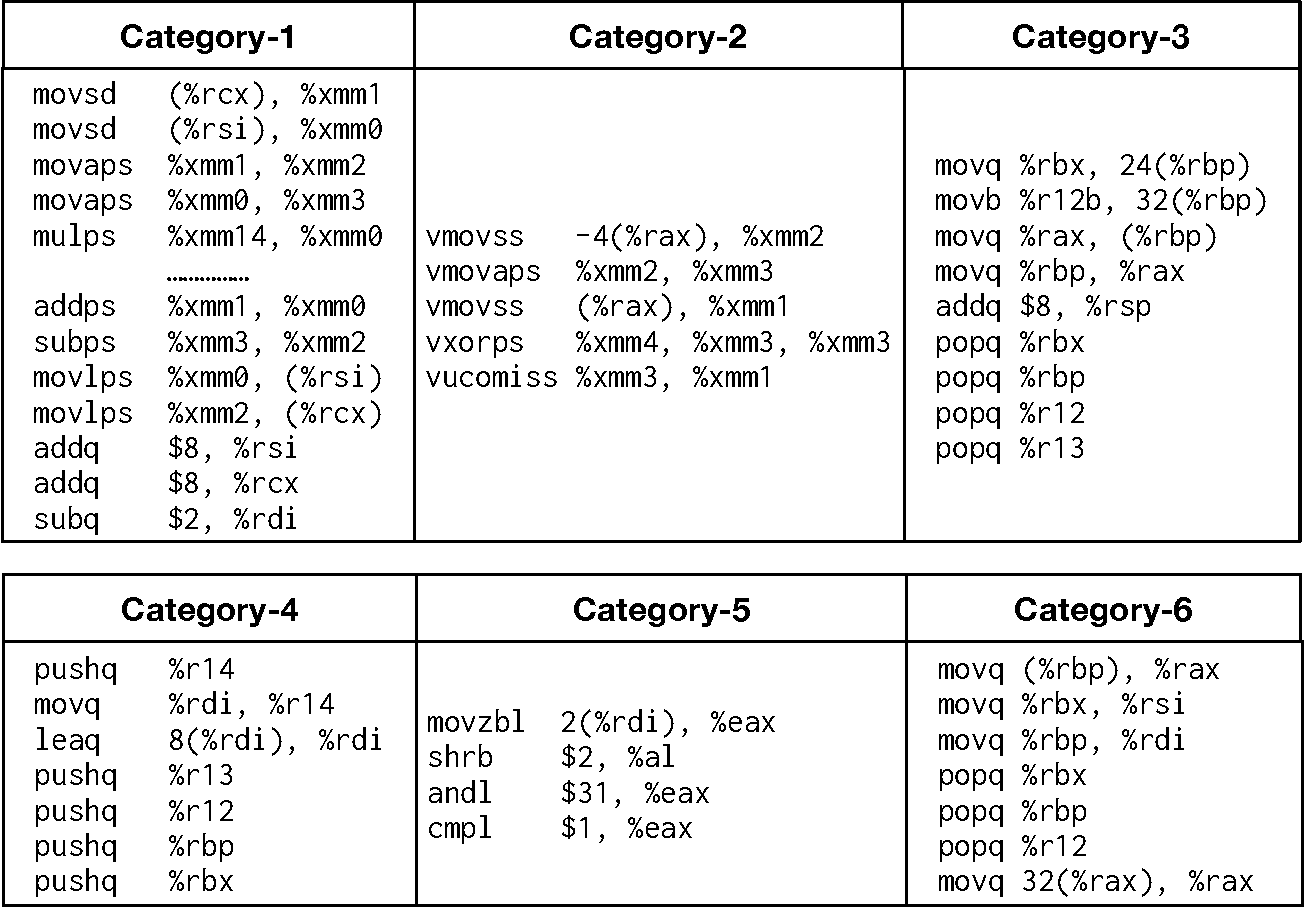
\includegraphics[width=\columnwidth]{figures/examples.pdf}
\caption{Example basic blocks for each category identified in Table~\ref{tab:categories}}
\label{fig:examples}
\end{center}
\end{figure}

% TODO: get a NICER figure
\begin{figure*}[h]
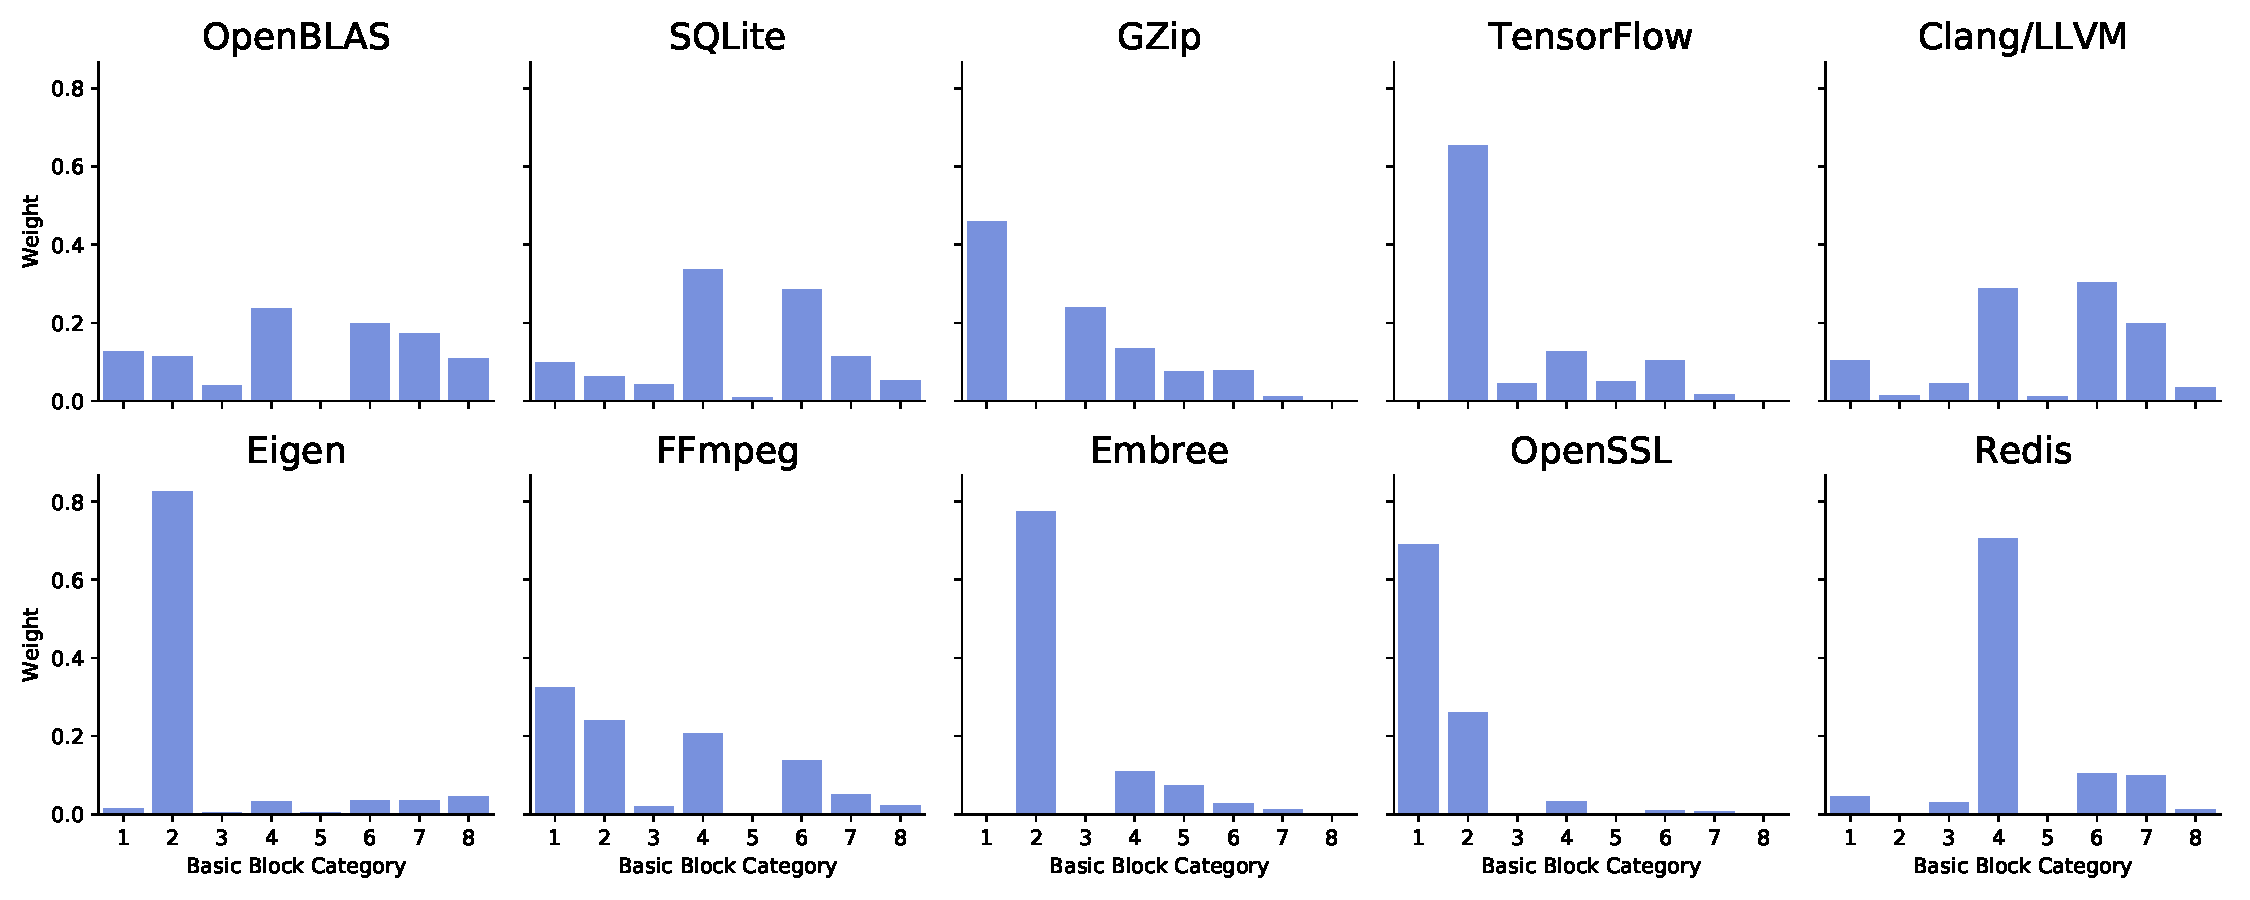
\includegraphics[width=\textwidth]{figures/apps-vs-clusters.pdf}
\caption{Breakdown of applications by basic block categories. The Y-axis is the percentage of basic blocks with the category specified on the X-axis. We define the category of a basic block as the most common category of micro-ops contained in the block.
Category-2 contains vectorized basic blocks.}
\label{fig:apps_vs_clusters}
\end{figure*}
\section{Results}

\subsection{Evaluation of Existing Models}
We evaluated IACA, llvm-mca, Ithemal\cite{ithemal}, and OSACA\cite{osaca}
on three recent Intel microarchitectures: Ivy Bridge, Haswell, Skylake.
Some basic blocks in our dataset contains AVX2 instructions, which are not supported in Ivy Bridge,
and these basic blocks are not included in validation for Ivy Bridge.
We use relative error (i.e. absolute error of the predicted throughput normalized by the measured throughput)
as the metric to measure inaccuracy.
Table \ref{tab:overall} shows the unweighted average error
of each model on different microarchitectures.
% include ivb and skl
Figures \ref{fig:ivb-app-err}, \ref{fig:hsw-app-err}, and \ref{fig:skl-app-err}
show the breakdown of the errors by applications.
Figure \ref{fig:ivb-cluster-err}, \ref{fig:hsw-cluster-err}, 
and \ref{fig:skl-cluster-err} show the breakdown of the errors by basic block categories 
(see \ref{classification} for details of basic blocks classification).
We note that the overall error of each model can be unrepresentative
of its performance on a given domain.
The discrepancy between these models' overall unweighted accuracy
and that of specialized domains (e.g. numerical kernels) highlights
the need of basic block classification and per-class error reporting.

Generally speaking, basic blocks dominated by stores
(category-4) are easier to predict,
while the throughput of basic blocks that mixes load instructions
with other operations (e.g. category-8) are considerably
more difficult to predict -- the prediction error is on average more than
twice higher than predicting basic blocks with only stores. 
We surmise that this is due to weakness of existing analyzers to model 
memory dependence.
In addition to basic blocks with memory dependence,
vectorized basic blocks (e.g. category-2) also causes high prediction errors.

% TODO summarize error by applications

\textbf{IACA}~\cite{iaca} is relatively more stable compared to other models that we evaluated.
An interesting point to note is that IACA is consistently accurate on basic blocks from OpenSSL.

\textbf{llvm-mca} is on par with IACA on Ivy Bridge and Haswell but considerably worse on Skylake,
especially on modelling basic blocks involving basic arithmetic operations.
We suspect the decrease in performance in Skylake is a result of LLVM developers 
having less time updating the cost models for the relatively new microarchitecture.

\textbf{Ithemal}~\cite{ithemal} consistently outperforms other models, except on vectorized basic blocks (i.e. category-2).
Ithemal is also considerably better than other models at modelling basic blocks with memory dependence,
as demonstrated by its errors on predicting basic blocks from categories 4 and 8.
We discussed ithemal's underformance on vectorized basic blocks with the authors of Ithemal, who suggested that the inconsistency
was a result of imbalance in their training dataset;
the majority of which, similar to our data set, consists of non-vectorized basic blocks.
In addition, the authors of Ithemal reported having to leave more basic blocks out of the training of their
Skylake model due to lack of reliable throughput measurements.
% TODO comapre error to basic block length and show ithemal does not generalize to large baisc blocks

\textbf{OSACA}\cite{osaca} generally has higher errors compared to other models.
We note that this might have less to do with OSACA's methodology than the engineering of its instruction parser.
During our evaluations, we found and reported five bugs related to OSACA's instruction parser.
In particular, OSACA does not recognize several instruction forms;
depends on the cases, it either crashes or treats unrecognized instruction forms as nops.
One such instruction form is any instruction that reads an immediate operand and writes to memory
(e.g. \verb|add [rbx], 1|), and OSACA treats these instructions as nops, thus under-reporting the throughput of
many basic blocks.


\begin{table}
\begin{tabular}{|p{0.25\columnwidth}|p{0.3\columnwidth}|p{0.25\columnwidth}|}
\hline

Microarchitecture & Model & Average Error\\
\hline

Ivy Bridge & IACA & 0.1693\\
    & llvm-mca & 0.1885\\
    & Ithemal & 0.1180\\
    & OSACA & 0.3277\\
\hline

Haswell & IACA & 0.1798\\
    & llvm-mca & 0.1832\\
    & Ithemal & 0.1253\\
    & OSACA & 0.3916\\
    
\hline 
Skylake & IACA & 0.1578\\
    & llvm-mca & 0.2278\\
    & Ithemal & 0.1191\\
    & OSACA & 0.3768\\

\hline
% TODO more for IVB and SKL
\end{tabular}
\\
\caption{Overall error of evaluated models.}
\label{tab:overall}
\end{table}

\begin{figure}
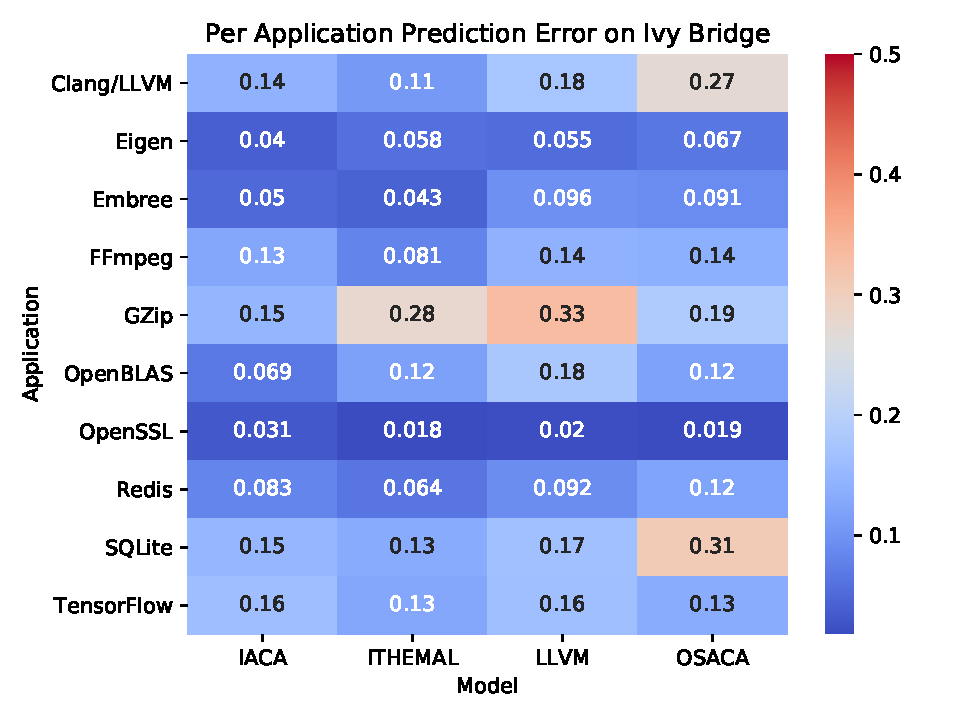
\includegraphics[width=\columnwidth]{figures/ivb-app-err.pdf}
\caption{Per-application error for each model on Ivy Bridge;
error for each basic block is weighted by the frequency it is sampled during profiling.}
\label{fig:ivb-app-err}
\end{figure}

\begin{figure}
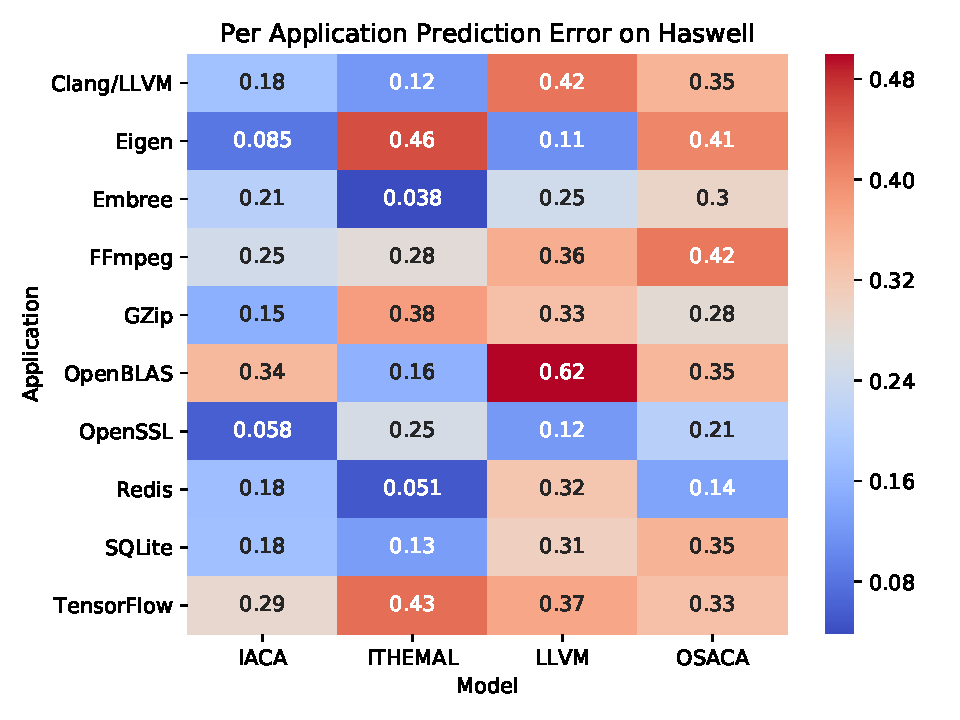
\includegraphics[width=\columnwidth]{figures/hsw-app-err.pdf}
\caption{Per-application error for each model on Haswell}
\label{fig:hsw-app-err}
\end{figure}

\begin{figure}
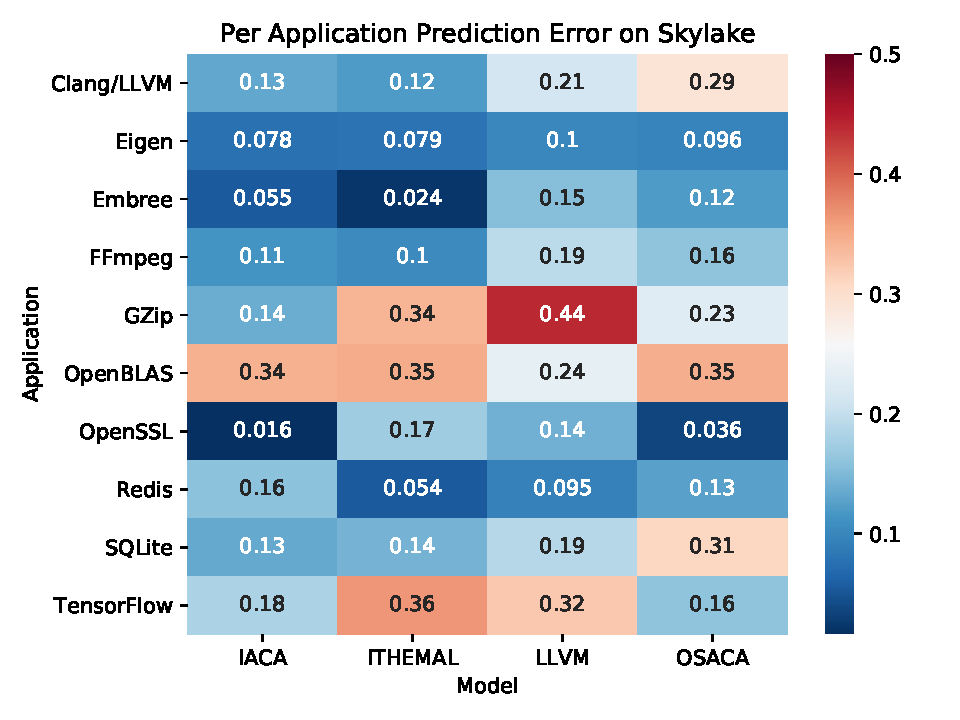
\includegraphics[width=\columnwidth]{figures/skl-app-err.pdf}
\caption{Per-application error for each model on Skylake. }
\label{fig:skl-app-err}
\end{figure}

\begin{figure}
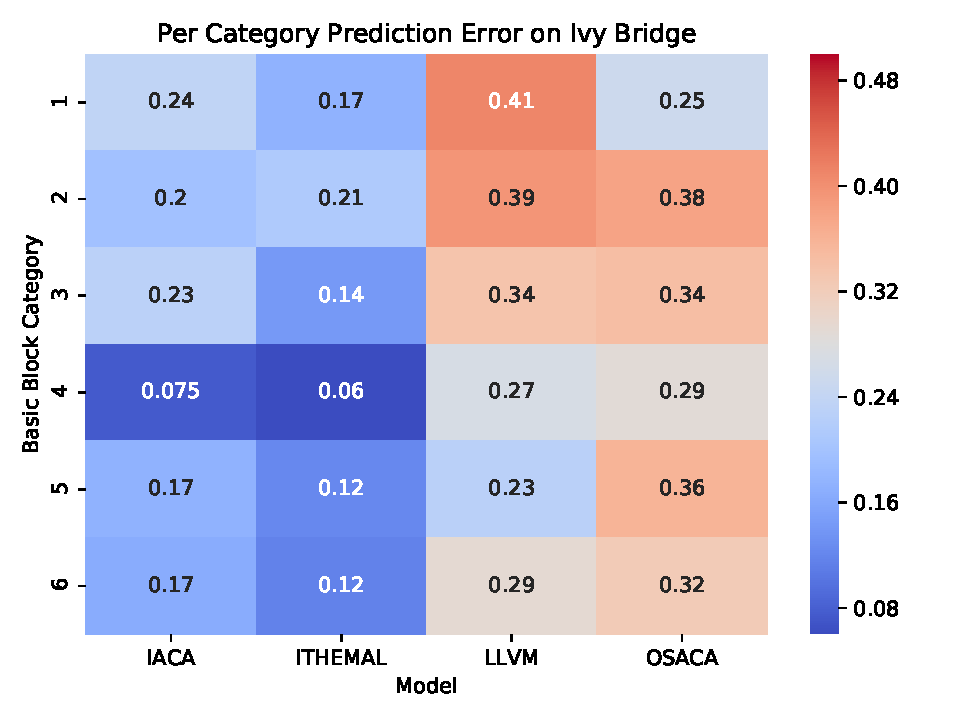
\includegraphics[width=\columnwidth]{figures/ivb-cluster-err.pdf}
\caption{Per-cluster error for each model on Ivy Bridge}
\label{fig:ivb-cluster-err}
\end{figure}

\begin{figure}
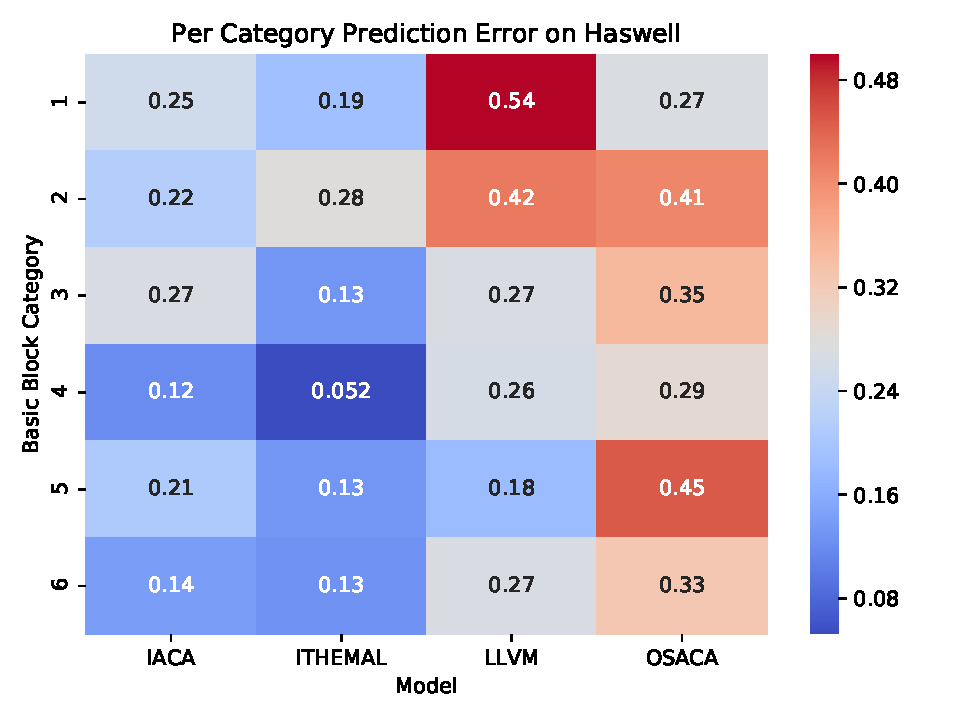
\includegraphics[width=\columnwidth]{figures/hsw-cluster-err.pdf}
\caption{Per-cluster error for each model on Haswell}
\label{fig:hsw-cluster-err}
\end{figure}

\begin{figure}
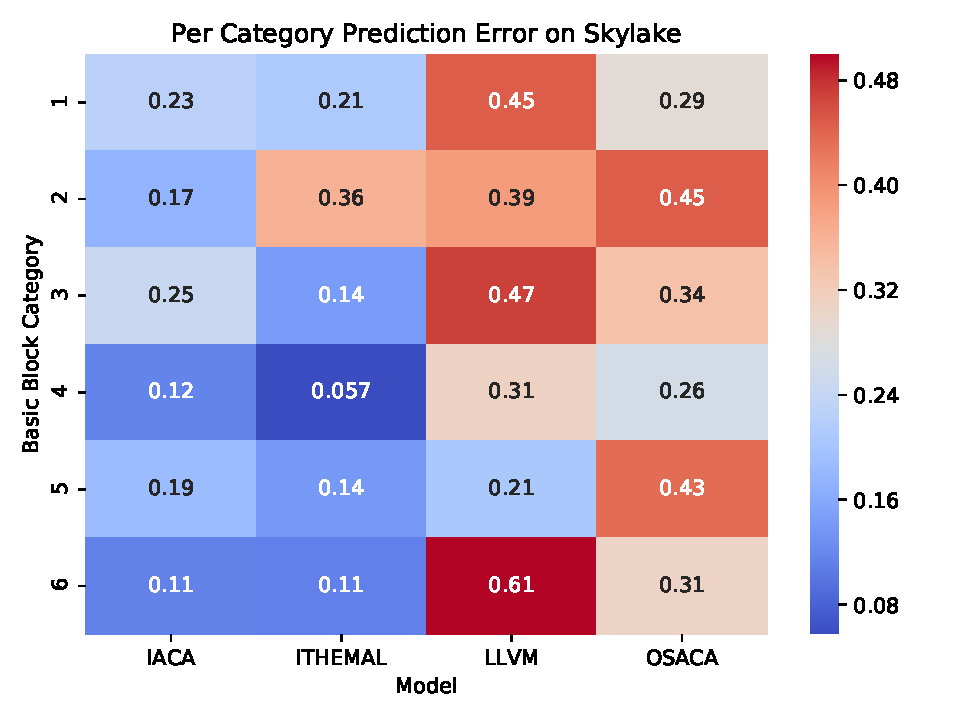
\includegraphics[width=\columnwidth]{figures/skl-cluster-err.pdf}
\caption{Per-cluster error for each model on Skylake}
\label{fig:skl-cluster-err}
\end{figure} 

\subsection{Interesting Basic Blocks}
We look at three basic blocks where some of the evaluated models behave poorly.
These results are from Haswell.
Table~\ref{tab:case-study} shows assembly of these basic blocks, their 
measured throughput, and throughput predicted by different models.
We manually inspected the instruction schedules predicted by the models
(except for Ithemal predicts a single throughput).
The first two examples highlights cases of some models' mis-prediction
contradicting instruction throughput specified by the manual.
The last example shows a case where a model (llvm-mca~\cite{llvm-mca} in this case) can significantly
mispredict throughput due to mis-scheduling, despite correct modeling of individual instructions.

\textbf{Modelling bug due to unsigned division}.
We look at the first example in Table~\ref{tab:case-study},
which is bottlenecked by a 64-bit by 32-bit unsigned division.
Intel's manual~\cite{intel-manual} states that the throughput of such division
ranges approximately from 20 to 26 cycles, which is consistent with our measurement (21.62).
All models are wrong here; llvm-mca and IACA~\cite{iaca} significantly over-predicts;
ithemal and OSACA~\cite{osaca} under-predicts.
llvm-mca and IACA's predictions indicate that they are confusing 
this division (\verb|div %ecx|) with the 128-bit by 64-bit analog (\verb|div %rcx|),
which the manual does specify to have variable latency between 80 and 95 cycles.
We note that the predictions made by llvm-mca and IACA would still be wrong
were we to replace the \verb|div %ecx| with \verb|div %rcx|,
due to the fast-path for zeroed out \verb|%rdx|.
(which is always the case here because of the preceding \verb|xor %edx, %edx|).

\textbf{Modelling bug due to zero-idioms}.
We look at the second example in Table~\ref{tab:case-study}.
The basic block consists of a single vectorized XOR of \verb|%xmm2| with itself.
All three micro-architectures we evaluated have fast-path for such zero-idiom.
IACA and Ithemal recognize this idiom and makes predictions close to the measured throughput,
while llvm-mca and OSACA treats this instruction as a regular vectorized XOR.

\textbf{Modeling bug due to mis-scheduling}
The last example in Table~\ref{tab:case-study} is the same basic block
we used as the motivating example in Section~\ref{sec:mapping}.
We focus on the schedule predicted by llvm-mca~\cite{llvm-mca}
and explain why llvm-mca overpredicts.
Figure~\ref{fig:schedule} shows the schedules predicted by llvm-mca and IACA.
Notice that the \verb|xorb| is dispatched for execution noticeably earlier in IACA's schedule.
llvm-mca delays the dispatch of this \verb|xorb| due to its dependence on the previous \verb|xorq|.
llvm-mca is unable to recognize that 
\verb|xorb -1(%rdi), %al| is implemented with a load micro-op followed by an ALU micro-op.
Since the load is independent, the hardware is able to schedule it ahead of time,
hiding its latency completely.
IACA is able to use this fact and predicts accurately.

\begin{figure}[htbp!]
    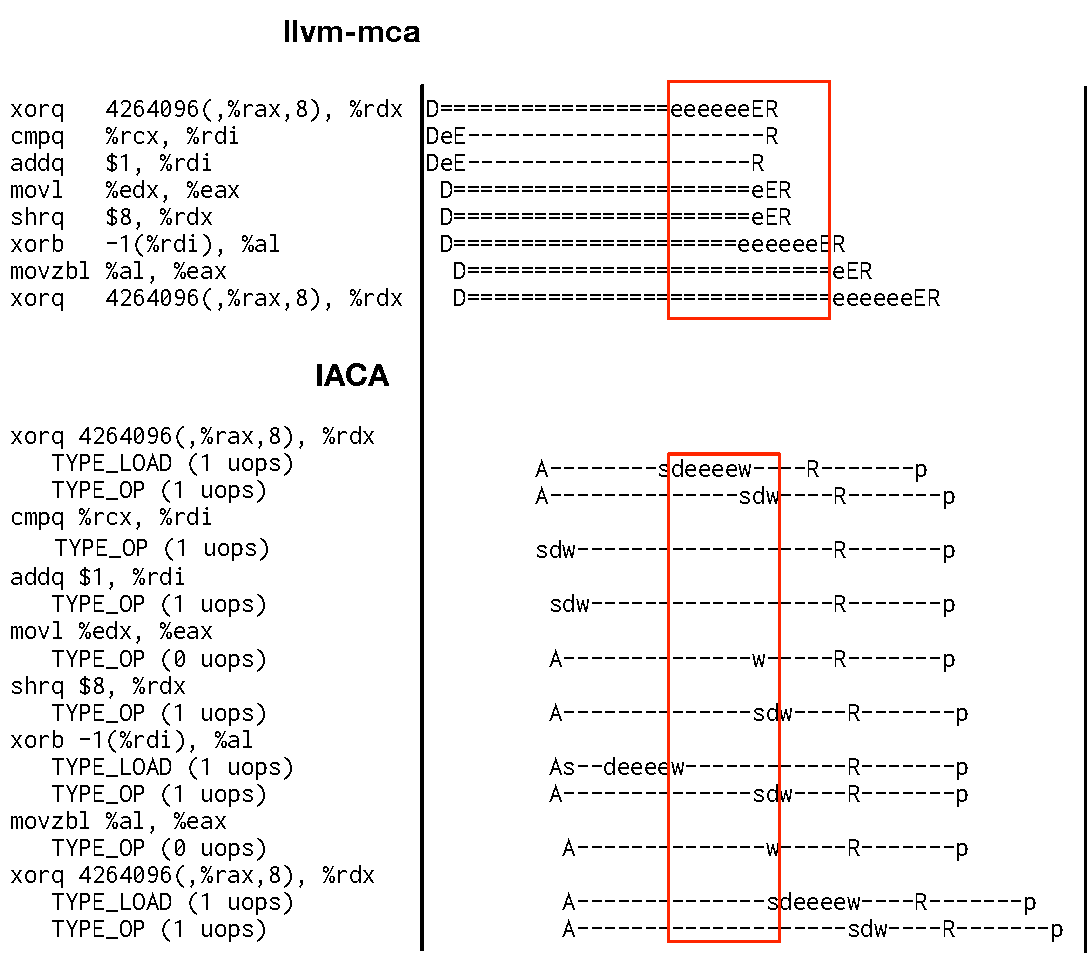
\includegraphics[width=0.95\columnwidth]{figures/scheduling.pdf}
    \caption{Schedules predicted by llvm-mca and IACA for an example basic block.
    Each red window marks the boundary of a single iteration of execution.
    The width of the windows represents the steady state throughput.
    As illustrated here, llvm-mca and IACA predicts two different schedules.
    Notice that the xorb instruction is dispatched earlier in IACA's schedules than in llvm-mca's. 
    }
    \label{tab:case-study}
\end{figure}

\begin{figure}[htbp!]
    \begin{center}
    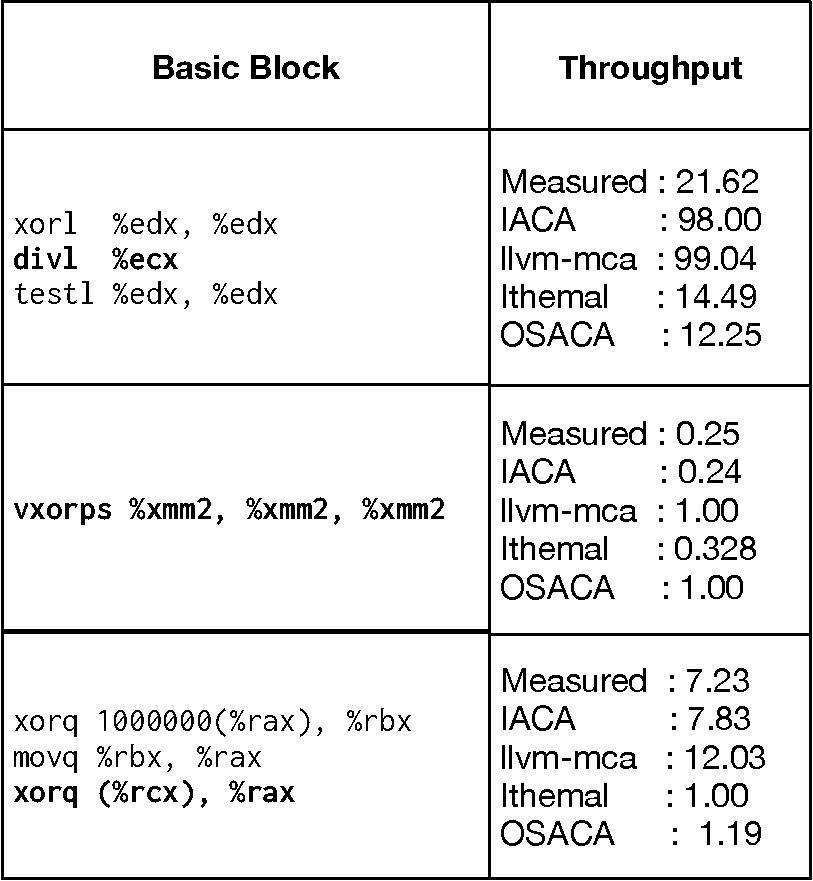
\includegraphics[width=0.7\columnwidth]{figures/interesting-examples.pdf}
    \caption{Interesting basic blocks and their inverse throughput as observed from measurements and reported by IACA, llvm-mca and OSACA (- indicates that the tool could not time the particular basic block).}
    \label{tab:case-study}
    \label{fig:schedule}
    \end{center}
\end{figure}

\begin{comment}
\begin{table*}[t]
    \centering
    \begin{tabular}{|l|c|c|c|c|c|}
    \hline
        Basic Block & Measured & IACA & llvm-mca & Ithemal & OSACA \\
\hline
\begin{lstlisting}
xor edx, edx
div ecx
test edx, edx
\end{lstlisting}
& 21.62 & 98.00 & 99.04 & 14.49 & 12.25 \\ 
\hline

\begin{lstlisting}
vxorps	 xmm2, xmm2,  xmm2
\end{lstlisting}
& 0.25 & 0.24 & 1.00 & 0.328 & 1.00 \\ 
\hline

\begin{lstlisting}
add rdi, 1
mov eax, edx
shr rdx, 8
xor al, [rdi - 1]
movzx eax, al
xor rdx, [8*rax + 0x4110a]
cmp rdi, rcx
\end{lstlisting}
& 8.25 & 8.00 & 13.04 & 2.13 & - \\ 
\hline 
    \end{tabular} 
    \\
    ~\\
    \caption{Interesting basic blocks and their inverse throughputs as observed from measurements and reported by IACA, llvm-mca and OSACA (- indicates that the tool could not time the particular basic block).}
    \label{tab:case-study}
\end{table*}
\end{comment}
\section{Conclusions}
We present a benchmark for validating throughput model of x86-64 basic blocks.
We describe the techniques with which we collected
and profiled 300,000 basic blocks from real-world applications.
Our benchmark can be used to systematically evaluate and tune performance models
of x86-64 basic blocks.
We evaluated four throughput prediction models, including two recently
published research models.
Our evaluation shows that even the best models we evaluated can differ from
the ground truth by more than 20\%, and sometimes more, 
for certain classes of basic blocks;
in particular, we show that existing throughput predictors have difficulty 
modelling memory dependency and vectorized basic blocks reliably.

\bibliographystyle{ieeetr}
\bibliography{paper}

\vspace{12pt}

\end{document}